\documentclass[a4paper,11pt]{style-esi/td}

\usepackage{style-esi/licence}
\usepackage{style-esi/exercice}
\usepackage{style-esi/exemple}
\usepackage{style-esi/question}
\usepackage{style-esi/tutoriel}
\usepackage{style-esi/listing}
\usepackage{style-esi/images}
\usepackage{style-dev1/dev1}

\begin{document}

\seance{Complément}{L'éditeur \bsc{VI}}
\libelledocument{\unitnb{} -- \unitname}
\entete
\titre
\ccbysa{esi-dev1-list@he2b.be}
\lastedit

\bigskip
% \tableofcontents

\section{L'éditeur \texttt{vi}}
%==================================

Dans le TD3, vous avez appris à utiliser l'éditeur \bsc{nano}.
Vous serez peut-être curieux d'apprendre à utiliser \texttt{vi},
un autre éditeur omniprésent sur \samp{linux1}.

Quels sont les avantages de \texttt{vi} ?
\begin{itemize}
	\item
	      Certaines manipulations du fichiers sont plus simples :
	      copier, supprimer, déplacer des lignes par exemple.
	\item
	      Il est facile d'indenter proprement un programme Java qui ne l'est pas.
\end{itemize}

\texttt{vi} est plus puissant que \texttt{nano}
mais il est moins intuitif quand on débute.
Voici les bases à comprendre.

\subsection*{Démarrer}
%========================

Pour éditer un fichier texte existant
ou créer un nouveau fichier,
il suffit de taper : \kbd{vi monFichier}.

Les 3 modes de fonctionnement sous vi(m) :
\begin{center}
	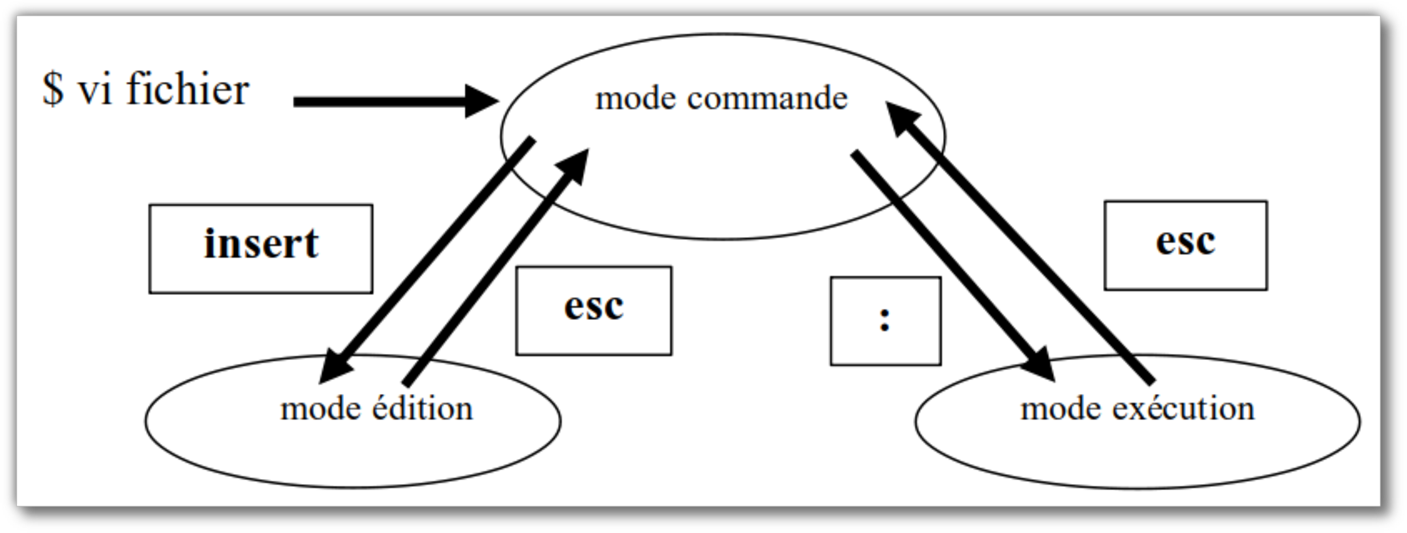
\includegraphics[width=.7\textwidth]{image/vi.pdf}
\end{center}

\subsection*{Le mode commande}
%===============================

C'est le mode dans lequel vous vous trouvez quand vous ouvrez \samp{vi}.
Dans ce mode, les touches sur lesquelles vous appuyez
ne sont pas insérées dans le texte (comme dans nano)
mais sont considérées comme des commandes.
C'est le mode qui permet de \textbf{manipuler} le texte.

Exemples de commandes :
\begin{itemize}
	\item \kbd{i} : passer en mode édition (cfr. infra);
	\item \kbd{yy} : copier la ligne sous le curseur (comme un \samp{CTRL-C} sous Windows) ;
	\item \kbd{3yy}	: copier 3 lignes ;
	\item \kbd{dd} : couper la ligne sous le curseur (\kbd{5yy} pour en couper 5) ;
	\item \kbd{dw} : couper le mot sur lequel se trouve le curseur ;
	\item \kbd{p} : coller (ce qui a été précédemment copié ou coupé)
	      sous la ligne qui suit le curseur ;
	\item \kbd{u} : annuler la dernière modification.
	      Vous pouvez appuyer plusieurs fois pour annuler les dernières modifications.
\end{itemize}

\subsection*{Le mode édition}
%===============================

C'est le mode dans lequel ce qu'on tape est ajouté au texte,
comme dans nano.
On y accède par la touche :
\begin{itemize}
	\item \kbd{i} (insert) : on insère à l'endroit du curseur ;
	\item \kbd{a} (append) : on insère après le curseur ;
	\item \kbd{o} : on insère dans une nouvelle ligne créée sous le curseur ;
\end{itemize}

Dans tous les cas, l'indicateur \texttt{INSERT}
apparait alors en bas de l'écran.

\subsection*{Le mode exécution}
%===============================

On y accède à partir du mode commande en tapant \kbd{:}.
Ce mode permet d'entrer d'autres types de commandes,
plus riches que celles du mode commande.
Voici les plus utilisées:
\begin{itemize}
	\item \kbd{:h} pour accéder à l'aide (\kbd{q} pour quitter l'aide) ;
	\item \kbd{:w} pour sauver le fichier ;
	\item \kbd{:w monFichier} pour enregistrer sous \samp{monFichier},
	\item \kbd{:q} pour quitter l'éditeur (sans sauver) ;
	\item \kbd{:x} pour enregistrer et quitter ;
	\item \kbd{:q!} pour quitter sans enregistrer les modifications ;
	\item \kbd{:set nu} pour afficher les numéro de ligne
	      (\kbd{:set nonu} pour les retirer) ;
	\item \kbd{:numéroDeLigne} pour aller directement à cette ligne ;
	\item \kbd{:\%s/old/new/g}
	      pour remplacer toutes les occurrences de la chaine de caractères
	      \samp{old} par la chaine de caractère \samp{new}.
\end{itemize}

\subsection*{Configuration}
%===============================

L'éditeur \bsc{vi} se configure via le fichier \samp{.vimrc}.
Vous pouvez trouver les détails ici :
\url{https://geekeries.org/2016/12/configuration-de-vim/?cn-reloaded=1}

\subsection*{Comparaison \bsc{nano} vs \bsc{vi}}
%===============================

\begin{tabular}{|l|l|l|}
	\hline
	                           & nano                                  & vi                       \\
	\hline\hline
	édition d’un fichier       & nano brol.txt                         & vi brol.txt              \\
	configuration              & ~/.nanorc                             & ~/.vimrc                 \\
	coloration syntaxique      & include "/usr/share/nano/java.nanorc" & syntax on                \\
	utilisation de la souris   & set mouse                             & Par défaut               \\
	indentation automatique    & set autoindent                        & set autoindent           \\
	lignes numérotées          & set linenumbers                       & set number               \\
	afficher l'aide            & Ctrl + G                              & ESC:h                    \\
	couper la ligne de texte   & Ctrl + K                              & ESC dd                   \\
	coller la ligne de texte   & Ctrl + U                              & ESC p                    \\
	rechercher dans le fichier & Ctrl + W                              & ESC /mot clef            \\
	sauver le fichier          & Ctrl + O                              & ESC :w                   \\
	quitter                    & Ctrl + X + option de sauvegarde       & ESC :x (avec sauvegarde) \\
	                           &                                       & ESC :q! (sans sauver)    \\
	\hline
\end{tabular}
\end{document}
